\documentclass{beamer}
\usetheme{Metropolis}
\graphicspath{{../img/}}
	
\usepackage[backend=bibtex, style=numeric, maxbibnames = 99]{biblatex}
\addbibresource{references.bib}

\usepackage[compat=1.1.0]{tikz-feynman}
\usepackage{tikz}
\usepackage{caption}
\usepackage{subcaption}
\title{\Large Mathematical model for the concentration and electric potential profiles in a solution of electrolytes under a redox reaction}
%\subtitle{\large{}}
\author{by Agust\'in Escobar Blanc \\ Advisor: Enrique Mu\~noz}
\institute{Pontificia Universidad Cat\'olica de Chile\\ Instituto de F\'isica}
\date{\today}

\newcommand{\qty}[1]
{
	\left({#1}\right)
}




\begin{document}

\begin{frame}
\titlepage
\end{frame}

\begin{frame}
\frametitle{Outline}
\tableofcontents
\end{frame}

\section{Diffusion Of Electrolytes In Aqueous Solution }


\begin{frame}
\frametitle{Diffusion equation with external electric field}
\begin{columns}
	\column{0.5\textwidth}
	\begin{itemize}
	\item The problem of diffusion
			$$\frac{\partial C_s}{\partial t}(x,t) +\nabla \cdot \mathbf{N}_s(x,t) = 0.$$
	\item Electric potential due to charge distribution (electrolytes)
			$$\nabla^2\phi = - \frac{\rho(x,t)}{\epsilon \epsilon_0}.$$
	\end{itemize}
	Here	$\epsilon$ is water's permittivity and $\epsilon_0$ the permittivity of free space. $s = \pm$.

	\column{0.5\textwidth}
	\begin{figure}
	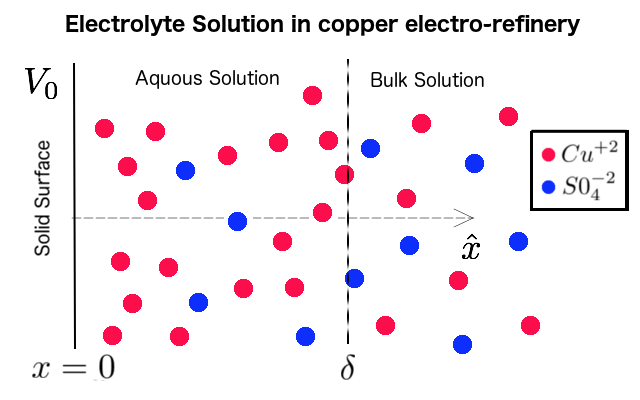
\includegraphics[width=\textwidth]{geometry.png}
	\caption{}
	\end{figure}
\end{columns}

\end{frame}

\begin{frame}
\frametitle{Mathematical model of the flux}
Model for the flux of electrolyte
$$\mathbf{N}_s= -D_s\left(\nabla\cdot C_s(x)_+ +s\frac{z F}{RT}C_s(x)\nabla\phi(x)\right)$$
 It is convenient to work with the dimensionless potential $\Psi = \frac{zF}{RT}\phi$
$$\mathbf{N}_s= -D_s\left(\nabla\cdot C_s(x)_+ +sC_s(x)\nabla\Psi(x)\right)$$

The charge distribution is given by the concentration of each electrolyte on every point of the solution times its electrical charge.
$$\rho(x,t) = \sum_{s = \pm} szFC_s(x,t)$$
\end{frame}





\begin{frame}
\frametitle{Mathematical model of the system}
Dimensionless length parameter $\xi = \kappa x$ 
Infinitely large plate implies $$\nabla_\xi^2 \rightarrow \frac{\partial^2}{\partial \xi^2}$$.  
With these considerations, the equations take the form

\begin{align}
\frac{\partial C_+}{\partial t}(\xi,t)  = - D_+ \nabla^2 C_s(\xi) - \nabla(C_+(\xi) \nabla \Psi(\xi,t)),\\
\frac{\partial C_-}{\partial t}(\xi,t) = - D_- \nabla^2 C_s(\xi) + \nabla(C_-(\xi) \nabla \Psi(\xi,t)),\\
\frac{\partial^2 \Psi(\xi,t)}{\partial \xi^2} = -\frac{\kappa^2}{C_b} \left(C_+(\xi,t) - C_-(\xi,t)_-\right).
\end{align}

where $\kappa^2 = \frac{(zFC_b)^2}{RT\epsilon_r \epsilon_0} $ and $C_b$ the bulk concentration.


\end{frame}

\begin{frame}
\frametitle{Border conditions}
\begin{columns}
	\column{0.6\textwidth}
	The border conditions for this problem can be obtained looking at figure \ref{fig:geometry2}
		\begin{itemize}
		\item $\qty{\partial C_+/\partial t + \nabla \cdot \mathbf{N_+}}\big|_{interface} = r$, 
		\item $\qty{\partial C_-/\partial t +  \nabla \cdot \mathbf{N_-}} \big|_{interface} = 0$, 
		\item $C_+ = C_- = C_b$,
		\item $\Phi(0) = \frac{zFV_0}{RT} = \Phi_0$ ,
		\item $\Phi(\delta) = 0$ .
	\end{itemize}		

	\column{0.4\textwidth}
	\begin{figure}
	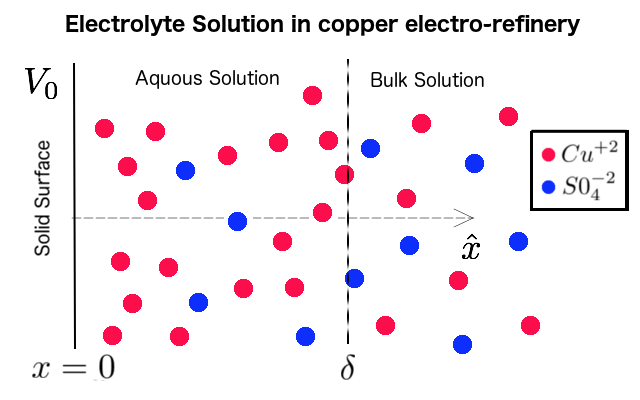
\includegraphics[width=\textwidth]{geometry.png}
	\caption{}
	\label{fig:geometry2}
	\end{figure}
	
\end{columns}
\end{frame}

\section{Steady State Solution}


\begin{frame}
\frametitle{Steady state approach}
As a first approach to solving the system, we compute the steady state solution.
\begin{align}
\frac{\partial C_+}{\partial t}(\xi,t)  = 0 &\Rightarrow \nabla \cdot\mathbf{N}_+ = 0& \Rightarrow \mathbf{N}_+(\xi)\big|_{surface} = r,  \\
\frac{\partial C_-}{\partial t}(\xi,t) = 0   &\Rightarrow \nabla \cdot\mathbf{N}_- = 0& \Rightarrow \mathbf{N}_-(\xi)\big|_{surface} = r, 
\label{eq:border}
\end{align}
which yields the following system of equations for the steady state problem
\begin{align}
\nabla C_+(\xi) - C_+(\xi) \nabla \Psi(\xi) = r, \\
C_-(\xi) +  C_-(\xi) \nabla \Psi(\xi) = 0, \\
\nabla^2 \Psi(\xi) = -\kappa^2 \left(C_+(\xi) - C_-(\xi)_-\right).
\end{align}
\end{frame}


\begin{frame}
\frametitle{Perturbation solution of the system}
By means of a perturbation analysis with $r$ as a control parameter we obtain solve the previous system up to first order in $r$. The zero order solution is
\begin{align}
\Phi^{(0)}(\xi) =  2\log{\qty{\tanh\qty{\frac{\xi-\xi_0}{2}}}},
\end{align}
Where
$$C^{(0)}_s(x)=C_{b,s}e^{s\Phi^{(0)}(x)}$$

\end{frame}

\begin{frame}
\frametitle{Perturbative solution of the system}
In order to solve the system to first order in $r$, the following approximation was made.
\begin{equation}
\bigg|\frac{\partial \phi^{(1)}}{\partial x}\bigg| << \frac{\kappa V_0}{r},
\end{equation}
Which yields
\begin{align}
C^{(1)}_+(\xi) &=& -\frac{1}{\kappa} e^{-\Phi^{(0)}(\xi)}\left(\xi-2\qty{\tanh\qty{\frac{\xi-\xi_0}{2}} + \tanh\qty{\frac{\xi_0}{2}}}\right)\nonumber,
\end{align}
and
\begin{align}
C^{(1)}_-(\xi) = 0.
\end{align}

\end{frame}


\begin{frame}
\frametitle{Analytic results for the concentration}
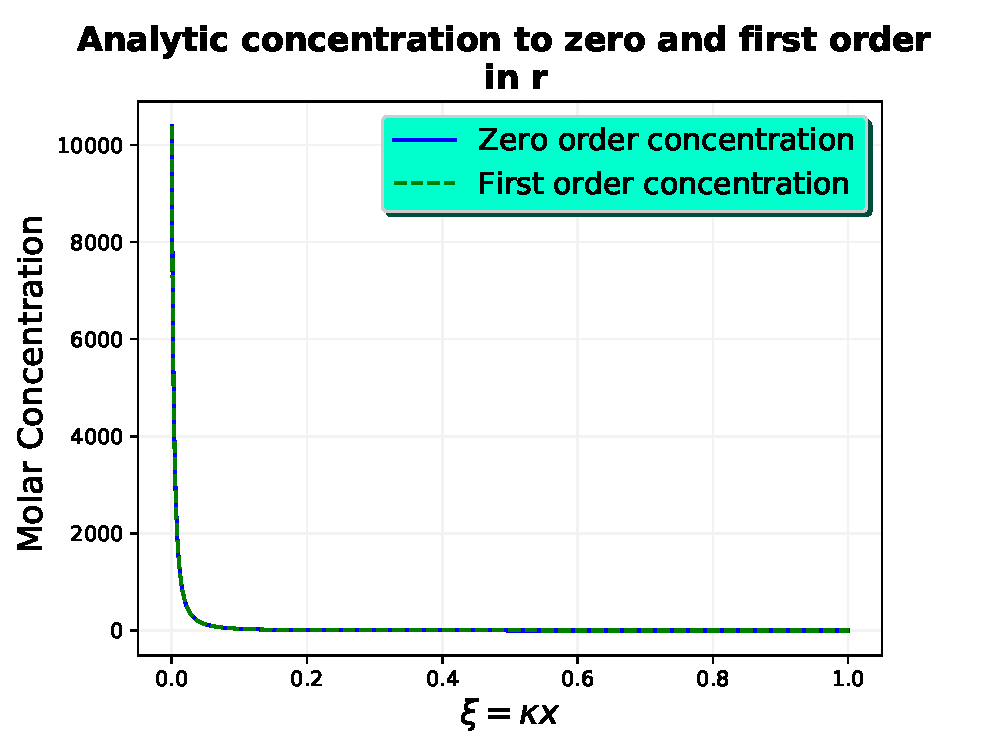
\includegraphics[width=\linewidth]{concentrations.eps}
\end{frame}

\begin{frame}
The first order term in the potential expansion is
\begin{align*}
\Phi'^{(1)}(\xi) = \frac{1}{\kappa} \qty{\frac{1}{2}\xi^2 -2\gamma \xi + 2(2\gamma-\xi)\coth\qty{\frac{\xi-\xi_0}{2}}} + C\\
C = -\frac{1}{\kappa} \qty{\frac{1}{2}\xi_\delta^2 -2\gamma \xi_\delta + 2(2\gamma-\xi_\delta)\coth\qty{\frac{\xi_\delta-\xi_0}{2}}}.
\end{align*}

\end{frame}

\begin{frame}
\frametitle{Analytic results for the potential}
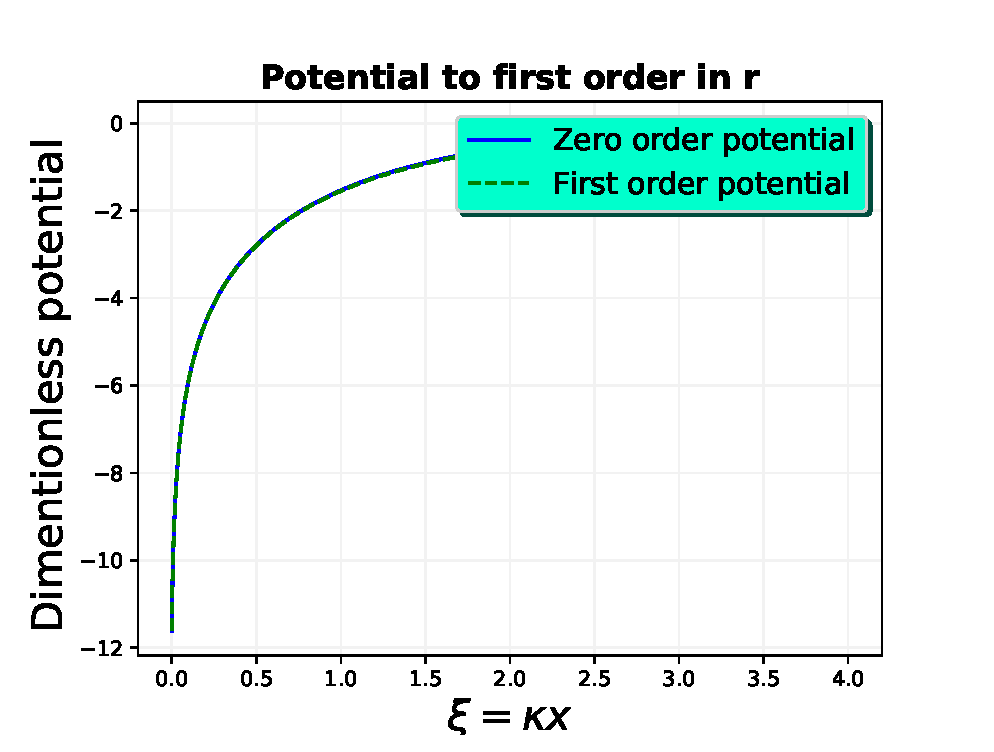
\includegraphics[width=\linewidth]{potentials-ana.eps}
\end{frame}



\begin{frame}
\frametitle{Numeric Results}
For numeric computation the Runge-Kutta of fourth order was used.  The following graph shows a comparison between the numeric an analytic system for $r = \kappa \times 10^{-5}\approx 2.28$.
\begin{center}
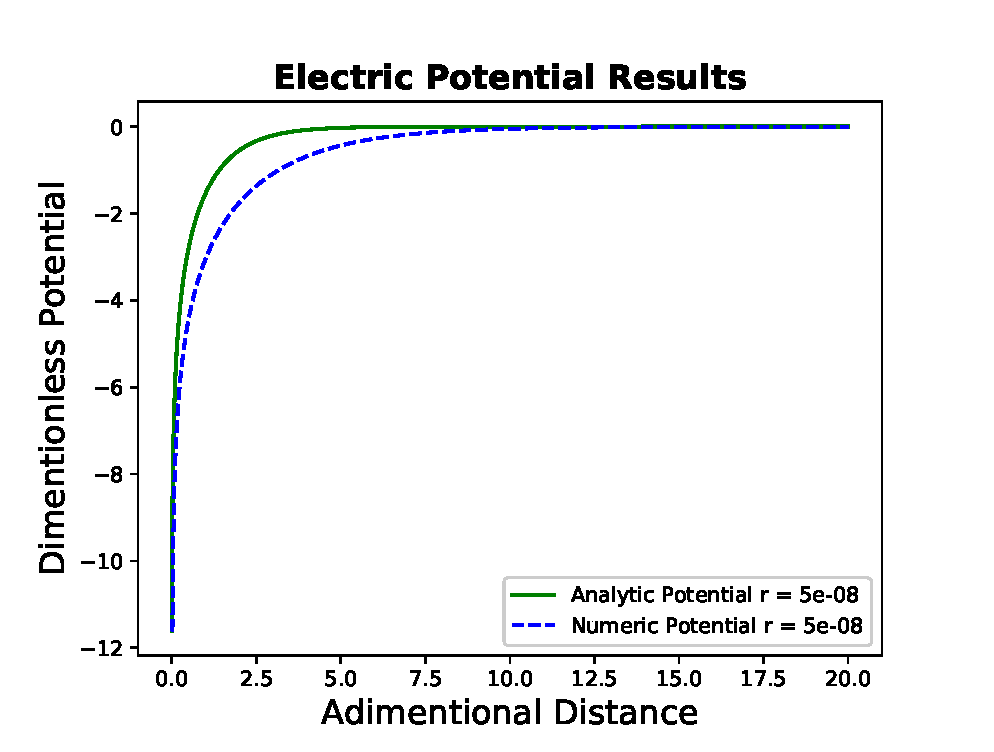
\includegraphics[width=0.7\linewidth]{potential-results.eps}
\end{center}

\end{frame}

\begin{frame}
\frametitle{Numeric Results}
The following graph shows a comparison between the numeric an analytic concentrations.
\begin{center}
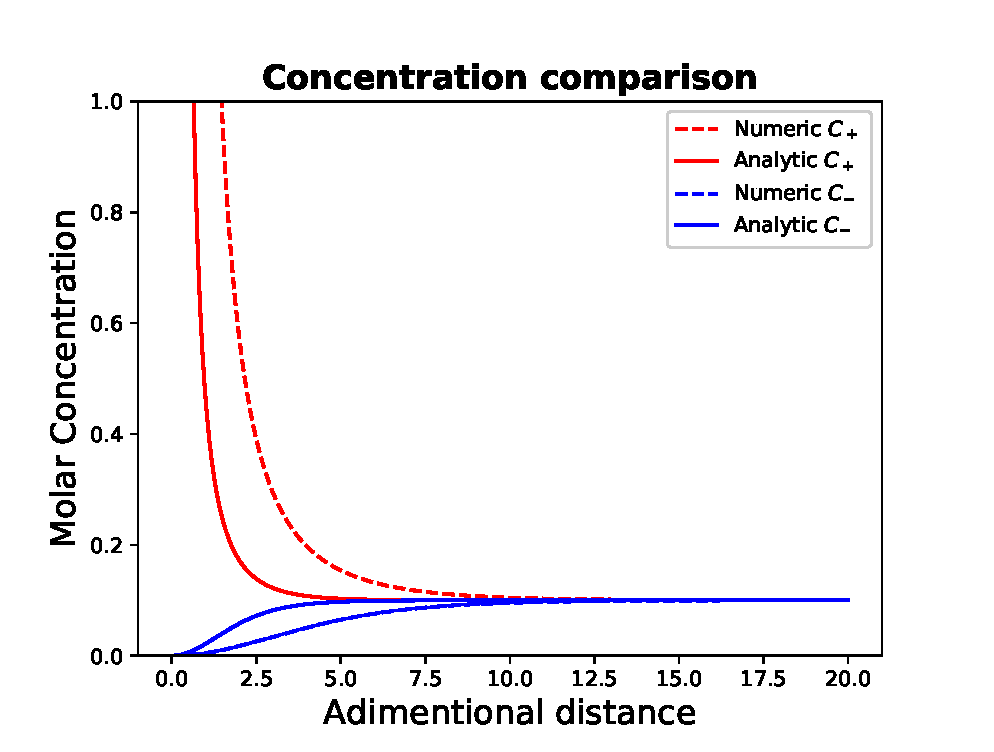
\includegraphics[width=0.7\linewidth]{Concentration-results.eps}
\end{center}
\end{frame}

\section{Dynamic solution}
\begin{frame}
\frametitle{Stage of the project}
We are currently working on solving the complete problem, including the dynamics. 
\begin{align}
\frac{\partial C_+}{\partial t}(\xi,t)  = - D_+ \nabla^2 C_s(\xi) - \nabla(C_+(\xi) \nabla \Psi(\xi,t)),\\
\frac{\partial C_-}{\partial t}(\xi,t) = - D_- \nabla^2 C_s(\xi) + \nabla(C_-(\xi) \nabla \Psi(\xi,t)),\\
\frac{\partial^2 \Psi(\xi,t)}{\partial \xi^2} = -\frac{\kappa^2}{C_b} \left(C_+(\xi,t) - C_-(\xi,t)_-\right).
\end{align}

\end{frame}

\begin{frame}
\frametitle{To-do list}
\begin{enumerate}
\item Finish numerical computation of the dynamical system
\item Include stochastic reaction rate to measure noise
\item Couple to NV-center. 
\end{enumerate}
\end{frame}


\end{document}



